\documentclass[runningheads]{llncs}
\usepackage{amssymb}
\setcounter{tocdepth}{3}
\usepackage{graphicx,epsfig}
\usepackage{algorithmic}
\usepackage{listings}
\usepackage{rotating}
\usepackage{subfigure}
\usepackage{multirow}
\usepackage[boxed]{algorithm2e}

\providecommand{\SetAlgoLined}{\SetLine}
\providecommand{\DontPrintSemicolon}{\dontprintsemicolon}
%%%%

\usepackage{color}
\usepackage{alltt}
\usepackage{verbatim}
\usepackage{url}
\usepackage[latin1]{inputenc}
%\usepackage[spanish]{babel}

%%

\usepackage{url}
\urldef{\mailsa}\path|pablogarcia@ugr.es|


\newcommand{\keywords}[1]{\par\addvspace\baselineskip
\noindent\keywordname\enspace\ignorespaces#1}

\lstset{
basicstyle=\ttfamily, %\scriptsize, QUITAR LA COMA DE TTFAMILY SI DESCOMENTAS
language=c++,
frame=single,
stringstyle=\ttfamily,
showstringspaces=false
}

\begin{document}
\pagestyle{empty} %ESTO QUITA LOS NUMEROS DE PAGINA
\mainmatter  % start of an individual contribution



% first the title is needed
\title{A methodology to develop services for Evolutionary Algorithms}


% a short form should be given in case it is too long for the running head
\titlerunning{A methodology to develop services for EAs}
\author{P. Garc\'ia-S\'anchez, A. M. Mora, P. A. Castillo, J. Gonz\'alez and J.J. Merelo}



\authorrunning{P. Garc\'ia-S\'anchez et al.}

% (feature abused for this document to repeat the title also on left hand pages)
% the affiliations are given next; don't give your e-mail address
% unless you accept that it will be published

\institute{Dept. of Computer Architecture and Technology and CITIC-UGR, University of Granada, Spain 
\mailsa}


\maketitle


\begin{abstract}
This paper proposes a methodology to design and implement Evolutionary Algorithms using Service Oriented Architecture. This paradigm allows to deal with some of the shortcomings in the Evolutionary Algorithms area, facilitating the development, integration, standardization and dynamism. A four-steps methodology to design services is presented: identification, specification, implementation and deployment. Also, as an example of application of this methodology, an adaptive algorithm is developed.
\end{abstract}



\section{Introduction}

Evolutionary Algorithms, and their subtypes (Genetic Algorithms, Evolution Strategies or Genetic Programming, among others) follow a number of common steps: initialization, evaluation, selection, recombination, mutation, replacement and stop criterion \cite{eiben2010whatis}. There exist many variations of these steps, and the different combinations can specify one algorithm or another. 

Distributed EAs can improve the algorithmic and computational performance over the non-parallel versions of the algorithms.
 Classic parallelization approaches \cite{alba2002parallelism}, such as the master-slave or island-based models, have been updated with the usage of new trends such as P2P \cite{laredo2010evag} or pool-based EAs \cite{meri2013cloud}. These new approaches manage with computational nodes entering and exiting during the experiment runtime and heterogeneous architectures.

Other research lines, such as the parameter adaptation or Memetic Algorithms \cite{ong2006classification} can imply the existence of some kind of dynamism involving the parts that compose an algorithm: for example, different recombinators or mutators working at the same time. Moreover, there exist several lines of parameter adaptation in dynamic and heterogeneous environments, where different computational elements are working at the same time.

Finally, there exist a large number of different (and incompatible) frameworks for EAs, each one using different languages, technologies and communication protocols. As Parejo et al. suggest  in \cite{SURVEYMOFS}, a standardization of these frameworks should be carried out. Moreover, it is difficult to access, in a public way, to available public systems to execute existent EAs to validate experiments and save time, encouraging Open Science \cite{Foster2005Science}.

Service Oriented Architecture (SOA) \cite{Papazoglou2007SOA} is a possible solution to deal with previous shortcomings. The elements that combine an EA are candidate to be designed as services, as they can behave as input/output functions. Also, SOA could help to solve the problems previously addressed: 

\begin{itemize}
\item {\em Development}: there exist several methodologies to model and design services. Also, as services are re-usable, they can be combined in different ways to create the different types of EAs. Moreover, existent technologies, also facilitate the development, using techniques such as versioning, packaging or life-cycle control.
\item {\em Integration}: Services are independent of the programming language. For example, services implemented in Java may use services implemented in C++ and vice-versa. Also, services allows distribution transparency: it is not mandatory to use a specific library for the distribution, or modify the code to adapt the existing operators. Existent EA frameworks could also be adapted to be accessed as services, providing their interfaces. 
\item {\em Standardization}: Interfaces of services use public standards (such as WSDL \cite{WSDL} or OSGi \cite{OSGI}). The service interfaces for EAs should be abstract enough to avoid their modification. Furthermore, as Foster claims \cite{Foster2005Science}, SOA is the key to develop Open Science.
\item {\em Dynamism}: Services are not aware of the order of execution, so this paradigm can fit with new parallel approaches for EAs, where the control of the nodes is not centralized. For example, new operators in different nodes can be bound and used during an algorithm's run. Also, there should be easy to add and remove elements to use the self-adaptation or other mechanisms.
\end{itemize} 

The rest of the work is structured as follows: after the state of the art, the description of our methodology is presented in Section \ref{sec:methodology}. Then, in Section \ref{sec:example} an example of application of the methodology to create a service oriented evolutionary algorithm is performed. The results of the created algorithm are shown in Section \ref{sec:results}. Finally, conclusions and future works are discussed.


%%%%%%%%%%%%%%%%%%%%%%%%SEC SOA
\section{State of the art}
\label{sec:soa}
The work of Gagn\'e and Parizeau \cite{GENERICITY05} established six criteria to qualify the genericity of a framework for EAs:  
 generic representation, generic fitness, generic operations, generic evolutionary model, parameter management and configurable output. These criteria should also been taken into account to develop service oriented evolutionary algorithms (SOEAs), that is, an evolutionary algorithm whose elements are services. A service is a loosely, coarse-grained, and autonomous component that allows interactions of all the elements that conform the system \cite{Papazoglou2007SOA}.

According to Valipour \cite{Valipour09surveysoa} services must follow these characteristics:

\begin{itemize}
\item {\em Discoverable and Dynamically Bound}: Services must be discoverable. Thanks to the service registry, a service consumer can discover a service to use at runtime.
\item {\em Self-Contained and Modular}: All functions in SOA are services. This means that every
  component in SOA must be modelled as a service, or as an aggregation of services. The services are well-defined: the interface of the service must be fixed, and it can not change in time, because the consumers or implementations of this interface should be modified with it. Services are, therefore, {\em encapsulated}: only the interface should be used to consume a service.
\item {\em Interoperability}: Consumers do not need to know how the service implementation performs their function, as services behave as a ``black box''. This is, elements such as the programming language or distribution protocol are independent.
\item {\em Loose Coupling}: Services should be designed to need only a few number of well-known dependencies.
\item {\em Location Transparency}: Services must be indistinguishably local or remote, being independent of the protocol to establish the connection.
\item {\em Composability}: Developing applications in SOA means to aggregate different existent services. Services are designed to be {\em re-usable}.
\end{itemize}

SOA has been previously used in the EA area. For example,
web services have been used in the grid area for optimization
problems, as can be seen in the works of
\cite{grid1}, where services are defined using WSDL
interfaces and other transmission mechanisms (such as Remote Procedure
Call \cite{grid6}). Although EAs are executed in grids
\cite{grid10}) no information about how to design these
services for EAs has been provided in previous works.

In our previous work \cite{Garcia13ServiceEAs}, an introduction to the usage of SOA to develop EAs, with some advantages, guidelines and examples was presented. However, that work does not count with a guided step by step methodology for EAs, as proposed in this paper.

\section{Methodology to develop services for EAs}
\label{sec:methodology}

This section presents all the steps to design and implement services for Evolutionary Algorithms. The selected steps have been adapted from SOMA \cite{Arsanjani2008SOMA}, a methodology to develop services focused in the business environments and adapted to be used in the EA research area.  As in SOMA, the phases of the proposed methodology are not linear, but they are iterative and incremental, that is, the designer can move back to a previous step if necessary. For example,
 new services can be discovered during the specification phase or changes on the specification could appear in the deployment phase. Figure \ref{fig:distributed:methodology} shows the steps of the proposed methodology.



\begin{figure}
\begin{center}
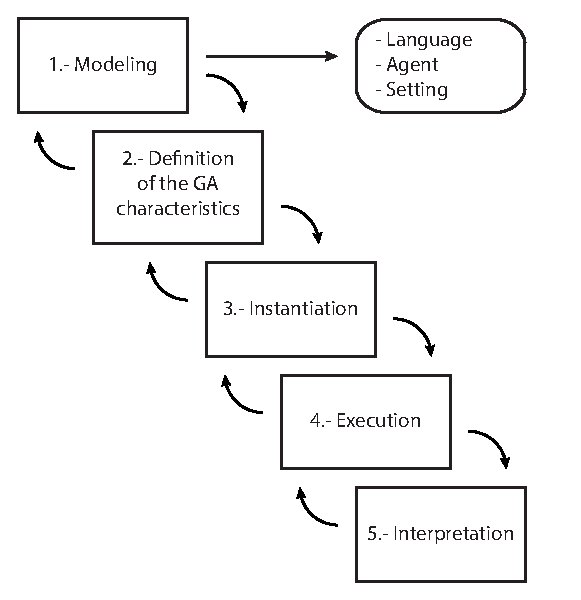
\includegraphics[scale=0.4]{methodology.eps}
\end{center} 
\caption{Methodology to develop services for Evolutionary Algorithms.}
\label{fig:distributed:methodology}
\end{figure}

\subsection{Identification}
\label{subsec:soaea:identification}

This phase is focused in the identification of the three constructs of SOA: services, components and flows. So, at the end of this step, the developers have a complete list of services to be designed.

First, the developers should ask themselves the following questions to facilitate the identification:
\begin{itemize}
\item Which problem I need to solve?
\item What elements need my EA?
\item Has somebody else programmed this before?
\item Which operators I need?
\item Is my algorithm going to be extended in the future?
\item How to parametrize my algorithm?
\end{itemize}

Solving the previous questions is the first step to identify the services. The next step is to classify the services in one of the three different domains are proposed. The three different domains are the {\em Algorithm domain}, the {\em Problem Domain} and the {\em Infrastructure Domain}. 

\subsubsection{Algorithm domain} Services in this domain are the ones that conform the EA. For example, operators of individuals, stop criterion, or populations.
 Getting the values of the parameters can also be a
  service,  thus the EA developer obtains two advantages over using the parameter only as variables: 
it is not mandatory to distribute the parameters among all services, and also they can be dynamically modified in execution time from an external service, facilitating self-adaptation.

\subsubsection{Problem domain} Services to address the elements of the problem. An example is the fitness function. The fitness function is a clear EA element that can be designed as a service. Each problem should implement an interface
  of the fitness service that receives the individual, allowing the
  distribution of this service (instead of being a method in the {\em individual} class, for example). Other services depends of the problem, for example an initializer of individuals.

\subsubsection{Infrastructure domain} Services in this domain are the ones that deals with the specific infrastructure that will be used. For example, services for user control, load balancing or logging. The design of many of these services is out of the scope of the EAs, but all them have to interact with the previous domains in some way. Depending of the environment where the EA is going to be developed other services needs to be modelled. For example, user control in cloud environments, different mechanisms for logging (in console, GUI...) or interconnection with other systems (such as external databases).

 

\subsection{Specification}

Once the services have been identified, the next step of the methodology establish the inputs and outputs of the services. The questions to solve prior to this phase are:

\begin{itemize}
\item Which are the inputs of the services?
\item Which are the operations of each service?
\item How the services are going to be used?
\item Which is the order of execution of the services?
\item Only one type of service is required?
\end{itemize}

 In this step all the characteristics of genericity for the design of an EAs \cite{GENERICITY05}, should be taken into account when designing elements for EAs. However, requirements are also aligned with the requirements for designing services \cite{Valipour09surveysoa}.


\subsubsection{Specifying the operators}
When specifying services such as 
{\em recombinator} or {\em mutator} they have to be modelled to not receive one or two
individuals, since not all EAs have the same behaviour. They should receive a
list of individuals to be crossed or mutated each generation. Almost all services in an EA (like mutation or selection) will accept individuals as input data and produce/modify these individuals. Due to many kind of individuals may exist, the operators should be as abstract as possible to operate properly. Therefore, services must accept {\em Individuals} interfaces as inputs, not concrete implementations, such as vectors or lists (generic representation). 

\subsubsection{Specifying the population} The population should not be a list of individuals: it should be a service
to access the individuals and allow the variation of its structure (for example, a change
from an unique list population to a cellular model) without
affecting  the rest of the pieces of the algorithm. So, other services
external to the EA could consult the {\em population} state and act
accordingly to some rules. 





\subsubsection{Specifying the fitness}




As in the operators, 
 the fitness should not be calculated within a method of an {\em Individual} class. To be less
coupled, it should be implemented an external service that receives a list of individuals (facilitating the load balancing). That way, the service is as abstract as possible. 

\subsubsection{Specifying the parameters}
Also the parameters should be a service for the same reason, allowing the possibility of performing
experiments related to  parameter control or tuning \cite{ParameterControlEiben07} in an efficient way
(being separated from the code of the existing operators). 

\subsubsection{Specifying the flow of the services}

An SOEA can be seen as a service flow. Flows should be designed to reducing the impact of potential future changes. An example of service flow would be an implementation called {\em Evolutionary Algorithm} with all the steps common to all EAs and with independence of the implementations of these steps (generic evolutionary model). This allow the adaptation of the evolutionary model. The user can manually
  select the services to be combined to create a Genetic Algorithm or
  an Evolution Strategy, for example.  

  Furthermore, to accomplish with the genericity presented by \cite{GENERICITY05}, the parameters and operators should be added dynamically. This is done with the SOA service binding. Users can specify the operators they need in several ways, for example, in a configuration file, or in an intelligent manner (an algorithm). It is important to remark that these ``pieces'' do not need to be modified and compiled again, because the loose coupling and the dynamic binding of SOA. Without SOA this behaviour is very difficult to achieve or maintain, as will be explained in next section.

\subsubsection{Specifying the infrastructure services}
The infrastructure services should be designed as flexible output mechanisms. For example, a GUI (Graphical User Interfaces) or logging should be independent of the services,  %FERGU: reescribe




It is important to remark that in the future these services could be extended, so they should be designed taking into account this possibility.

\subsection{Implementation and deployment}
\label{subsec:soaea:implementation}
Once the services have been identified and specified, a SOA technology should be used for implementing the services and publish them to be accessed. This two steps of the methodology are explained together because the decisions about the technological solution to be used is bound to both phases.

The questions to solve in this steps are:
\begin{itemize}
\item Services are going to be used locally or remotely?
\item How the interfaces are going to be exposed?
\item Are the services public?
\item How the changes in service dynamism are going to be managed?
\item How must be the overload of the messages? 
\item Which are the advantages of the chosen technology?
\item Which are the considerations about security, persistence, benchmarking and monitoring?
\end{itemize} 

\subsubsection{Select the technology to expose the interface}
As presented in the introduction there exist several technologies for implementing services. Depending of the use of the services, one technology should be chosen over other. For example, a service that is going to be used remotely and publicly from any programming language should export the interface with WSDL publicly available with an URL, to allow users automatically generate the client for that service. On the other side, interfaces are previously known, and it is not necessary to export them to the public. This is the case of OSGi, where the interface is exposed only to the OSGi service registry. Other mechanisms could be used to publish and share the interfaces of the services (for example, using a {\em newcast} protocol).

\subsubsection{Select the communication mechanism}
Services are also independent of the transmission mechanism, so this issue must be considered depending of the system to deploy the services. In the case of EAs, where the performance is important, usually the most efficient transmission mechanism should be preferred. However, sometimes other transmission mechanism can be used. For example, SOAP includes extra information in headers \cite{Castillo13SOAP}, producing more network overload. However, this information is more easy to manage for other systems, or easier to configure to be used remotely (as it uses standard HTTP port).

\subsubsection{Deploy in the system} 
Once the services have been implemented they have to be deployed in the desired system. In this step, issues related with testing, user control, security and persistence should be taken into account.




\section{Example of creating a service oriented evolutionary algorithm}
\label{sec:example}
This section justifies the use of SOA-EA and the steps to create services within it. In this example, a basic genetic algorithm to solve the MMDP problem \cite{goldberg92massive} will be designed. This algorithm needs to automatically bind new operators (not previously known by the algorithm) when the algorithm has found a local optimum. No extra code should be added to the algorithm to bind/unbind operators or check the population.


\subsubsection{Identification}
As  stated in introduction, a basic EA is formed by several steps. These steps are common to every EA, so this part should be fixed  to allow the creation of services as abstract as possible. Solving the questions in Section \ref{subsec:soaea:identification} and the considerations about the design of services \cite{Valipour09surveysoa} and the genericity of EAs \cite{GENERICITY05} a number of abstract services have been identified. In the {\em algorithm domain}, the Algorithm, Population, Parent Selector, Recombinator, Crossover, Mutator, Mutation, Replacer, Stop Criterion and Parameters. In the {\em problem domain}, the Fitness Calculator and Initializer. Finally, a {\em infrastructure domain} service called Asynchronous Enabler, who is in charge of activate new operators when a local optimum is found (for example, no changes in best individual during certain time).

\subsubsection{Specification}

 Concrete implementations are defined: {\em N Tournament} and {\em Roulette} are implementations of parent selectors and {\em Optimum Found} the desired stop criterion. Also, to address the problem to solve, such as {\em MMDP Fitness Calculator} or {\em Binary Initializer}. As we need a fixed set a Evolutionary, a {\em Evolutionary Algorithm} service is created to model the flow of services. The discovered services have been specified to accept  a list of individuals. A service to gather all selectors in the environment is used.

 Infrastructure services to deal with control of the population and enabling of other operators are also implemented (Asynchronous Enabler Impl). Figure \ref{fig:enabler} shows this designed configuration.

 \begin{figure}
\begin{center}
\includegraphics[scale=0.5]{enabler.eps}
\end{center} 
\caption{Automatic binding of new operators. White boxes are interfaces and orange boxes are implementations of the services.}
\label{fig:enabler}
\end{figure}

 \subsubsection{Implementation and Deployment}
 Because we require an automatic binding and asynchronous and parallel control of the population services OSGi is the technology proposed to implement this example. The services are deployed in an Equinox server. The reasons of using these technologies are explained in \cite{Garcia13ServiceEAs}, but summarizing, it allows automatically binding of implementations to interfaces without extra code or recompiling, and dynamic discovery of services, as this example requires. 

 Source code of the proposed implementation is available under a GNU/LGPL V3 in our repository at \url{http://www.osgiliath.org}.

\section{Experimental results}
\label{sec:results}

This section shows the results obtained comparing using the automatic enabling of operators. Two versions have been compared: a non-adaptive version that only uses a Binary Tournament for Selection, and an adaptive one, which automatically enables a Roulette Selection when a local optimum is found. The parameters used in this comparison (accessed from the Parameters service) are a population of 64 individuals, selector rate of 0.5, TPX crossover, bit flip mutation, and individual length of 60 elements. The Roulette selector is enabled when the best individual of the population has not changed in 10 seconds (checked every 2 seconds).

\begin{table}
\resizebox{11cm}{!}{
\begin{tabular}{|c|c|c|c|}
\hline
			 & Generations		  		& Evaluations			   		 & Time \\ \hline \hline
Non-adaptive & 219403,1 $\pm$ 141692,16 &	14041926,4	$\pm$ 9068298,82 & 68766,4 $\pm$ 45073,04	\\ \hline
Adaptive 	 & 167166,66 $\pm$ 93594,37 &	10698794,66	$\pm$ 5990039,68 & 51710,4 $\pm$ 29329,21 	\\ \hline
\end{tabular}
}
\caption{Results obtained.}
\label{tab:results}
\end{table}			

 \begin{figure}
\begin{center}
\includegraphics[scale=0.3]{datos.eps}
\end{center} 
\caption{Boxplot of the number of evaluations in each configuration.}
\label{fig:datos}
\end{figure}

As can be seen, automatic and adaptive enabling selection operators has an increase of performance, reducing time and evaluations (both significantly with a p-value$<$0.05 of a Wilcoxon test). It must be remarked that the aim of this work is not the numerical results obtained, but use this example to demonstrate that applying a methodology to develop loose coupled services that can be dynamically bound, without modification of the existent services can be used to achieve better results.

\section{Conclusions}
\label{sec:conclusion}

 There exist several shortcomings in the Evolutionary Algorithms area, such as the  incompatibility between frameworks or new trends of distributed programming, where nodes enter and exit in runtime, for example. All these facts  motivate the creation of a proper way to define services for evolutionary algorithms to facilitate the development, integration, standardization and dynamism.

In this paper the requirements in EA design (genericity in representation, fitness, operations, model, parameters and output) presented by Gagn� and Parizeau, with the requirements in SOA (genericity in interfaces, language independence, distribution and dynamism), have been taken into account to propose a methodology to model the services that compose a service oriented EA (SOEA), and several guidelines about the design of these services have been explained. This methodology proposes 4 iteratively and incremental phases: identification, specification, implementation and deployment. A number of questions to answer in each phase to help in the development has been proposed. This methodology has been used to create a service-oriented evolutionary algorithm that takes advantages of the SOA capabilities, such as loose-coupled services and automatic binding of new operators.

In future work, this methodology will be used to create new examples of SOEAs and refined to deal with other shortcomings. Other technologies available in SOA will also be tested and analysed.


\section*{Acknowledgements}
This work has been supported in part by FPU research grant AP2009-2942 and projects SIPESCA (G-GI3000/IDIF, under Programa Operativo FEDER de Andaluc�a 2007-2013), EvOrq (TIC-3903), CANUBE (CEI2013-P-14) and ANYSELF (TIN2011-28627-C04-02).

\bibliographystyle{splncs}
\bibliography{soaea}



\end{document}

